In a dense target environment, the gating technique is not sufficient enough to discriminate between detections. Thus a further assignment logic has to be implemented. Conflicts can occur for instance, when a detection satisfies the gating of different tracks, or when a track was multiple detections within its gate. This problem is called the assignment problem. 

There are basically two types of solutions. The  \ac{nn}-approach (\cref{mtt:nn}) and the "all-neighbors" approach (\cref{mtt:pda} and \cref{mtt:jpda}). The first step of all solutions, however, is the same. First, an assignment matrix is built. For this, the norm of the innovation vector that would result if track $i$ and detection $j$ would be assigned is defined as 

\begin{equation}
d_{ij}^2 \triangleq \vec{v}_{ij}(n)^T \matrix{S}_i^{-1}(n)\vec{v}_{ij}(n)\\,
\end{equation}
where $\matrix{S}_i(n)$ is the residual covariance matrix defined in \cref{eq:innov}. Furthermore, it is assumed that the residual has a Gaussian distribution
\begin{equation}
	g_{ij} =\frac{\exp(-\frac{d_{ij}^2}{2})}{(2\pi)^{M/2}\sqrt{|\matrix{S}_i|}}\\,
\end{equation}
where $M$ is the measurement dimension and $|\matrix{S}_i|$ the determinant of $\matrix{S}_i$.
\begin{figure}[h]
	\centering
	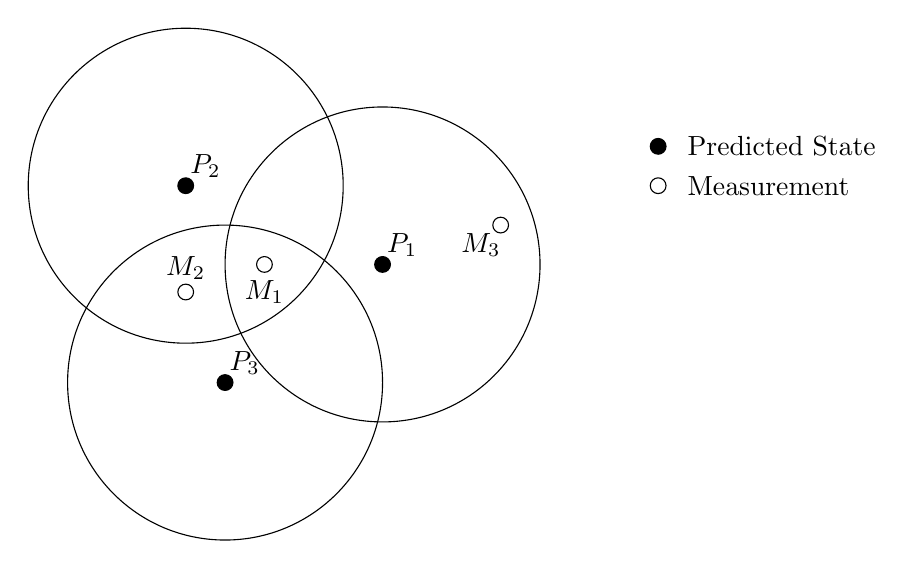
\begin{tikzpicture}

\draw[black, fill = black] (4.5,1.5) circle(0.1cm); 
\draw[black, fill = black] (2,2.5) circle(0.1cm); 
\draw[black, fill = black] (2.5,0) circle(0.1cm); 
\draw[black,] (4.5,1.5) circle(2cm); 
\draw[black,] (2,2.5) circle(2cm); 
\draw[black,] (2.5,0) circle(2cm);
\draw(4.75,1.75) node{$P_1$}; 
\draw(2.25,2.75) node{$P_2$}; 
\draw(2.75,0.25) node{$P_3$}; 

\draw[black] (3,1.5) circle(0.1cm); 
\draw[black] (2,1.15) circle(0.1cm); 
\draw[black] (6,2) circle (0.1cm); 


\draw(3,1.15) node{$M_1$}; 
\draw(2.,1.45) node{$M_2$}; 
\draw(5.75,1.75) node{$M_3$}; 

\draw[black, fill = black](8,3) circle(0.1cm); 
\draw[anchor = west](8.25,3) node{Predicted State}; 
\draw[black, ](8,2.5) circle(0.1cm); 
\draw[anchor = west](8.25,2.5) node{Measurement};





%\draw[black, fill = black](8,3) circle(0.1cm); 
%\draw[anchor = west](8.25,3) node{Predicted State}; 
%\draw[black, ](8,2.5) circle(0.1cm); 
%\draw[anchor = west](8.25,2.5) node{Measurement};
%\draw[black](8,2) circle(0.1cm); 
%\draw(8,2) node [cross,red] {}; 
%\draw[anchor = west](8.25,2) node{Discarded Measurement}; 


\end{tikzpicture}
	\caption{Example of conflict situations for assignment}
	\label{fig:assign}
\end{figure} 

The basic goal is to make assignment decisions based on the maximization of $g_{ij}$, which is equivalent to minimizing the quantity 
\begin{equation}
	d_{Gij}^2 = d_{ij}^2 + \ln |\matrix{S}_i|\\,
\end{equation}
which will be used as distance function for use in the assignment problem.

